\subsection{Network Metrics Analysis}
%\addcontentsline{toc}{subsection}{Network Metrics Analysis}%
As explained in the previous subsection, one can label a data set differently and generate identical graphs with \acs{fss} Network and \acs{fbs} Network approaches. We argue that resultant graphs have various motifs which are non-trivial and emerge from the statistical patterns in data. In further steps in this subsection, we review a well-known network measure: modularity and statistical techniques of randomness control to be integrated into our analysis pipeline.
\subsubsection*{Modularity Measure}
The variety of textures arises from how the nodes are clustered within their neighbourhood or having different degree values. The degree is a network metric that quantifies one node's links (or edges) to the other nodes~\cite{Barabasi2016}. The degree distribution of the network gives an idea about the connectivity patterns within the network. It allows us to distinguish the nodes with a high degree from the nodes with a low degree.

Identification of tightly connected node groups is a way of quantifying community structure in networks~\cite{Girvan7821}. Communities (the so-called modules) are groups of nodes that probably play similar roles within the graph~\cite{FORTUNATO201075}. Modularity is a network measure for community detection and quantifies the strength of community structure in that specific network. It is a way to express the network characteristics.

Newman (2006) formulated modularity in his article as
\begin{equation} %\tag{2}
	Q = \frac {1} {4 m}\sum_ {ij} (A_{ij} - \frac {k_{i} k_{j}}{2 m}) s_{i} s_{j} ,
	\label{modularity}
\end{equation}
\myequations{Modularity Formula} 
where the network graph has an $m$ number of edges, and $A_{ij}$ is the number of edges between vertices $i$ and $j$. $A_{ij}$ is the element of the adjacency matrix introduced in Fig.~\ref{figure-adjacency_graph}. It can be $0$ or $1$. $k_{i}$ and $k_{j}$ are the vertex degrees, and ${k_{i} k_{j}}/{2 m}$ is the expected number of edges between $i$ and $j$ if edges are randomly placed. $s_{i}$ and $s_{j}$ are the divided network groups. They are equal to $1$ if $i$ and $j$ belong to the same group and $0$ otherwise. Eq.\eqref{modularity} is used to separate the network into two communities only; however, many networks may contain more than two communities. Therefore, a repeated division into two is adapted: dividing the network into two graphs, then the two sub-graphs further divided into two only if that would maximise $Q$. After first partitioning, the edges falling between the further divided sub-graphs are neglected, leading to a wrong maximisation quantity. For this reason, the author introduced the additional contribution $\Delta Q$.~\cite{Newman8577}
% $B_{ij} = A_{ij} - \frac {k_ {i} k_ {j}} {2 m}$\\
% $Q = \frac {1} {4 m} s^{T} Bs = \frac {1} {4 m}\sum_ {i = 
%	1}^{n} (u_ {i}^{T} . s)^{2}\beta_ {i}$\\
% $\Delta Q = \frac {1} {4 m} s^{T} B^{(g)} s$\\
% $B_{ij}^{(g)} = B_{ij} - \delta_{ij}\sum_ {k\in g} B_{ik}$

The formulation given in Eq.\eqref{modularity} was used in this thesis work to calculate the modularity of the association networks. Since the results obtained with the combination of $Q$ and $\Delta Q$ do not significantly differ from the results obtained only using $Q$, the modularity calculations in this work were performed with the latter one to lower the computation timing.

\subsubsection*{Randomness Control Concerning Different Null Models}
As Eq.~\eqref{modularity} gives a clue, one can measure a real network modularity quality by comparing it with the community structure in a random graph~\cite{GirvanNewman2004}. The distribution of degrees in random graphs is highly homogeneous, and they do not reveal a significant level of order or organisation~\cite{FORTUNATO201075}. Various sophisticated random graphs (the so-called null models) can be generated from the original network graph by keeping some of its structural properties the same~\cite{Maslov910, MERTEN2020, FORTUNATO201075, Enders2018}.
 \begin{figure}[!ht]
	\begin{center}
		\makebox[\textwidth]{
			\centering
			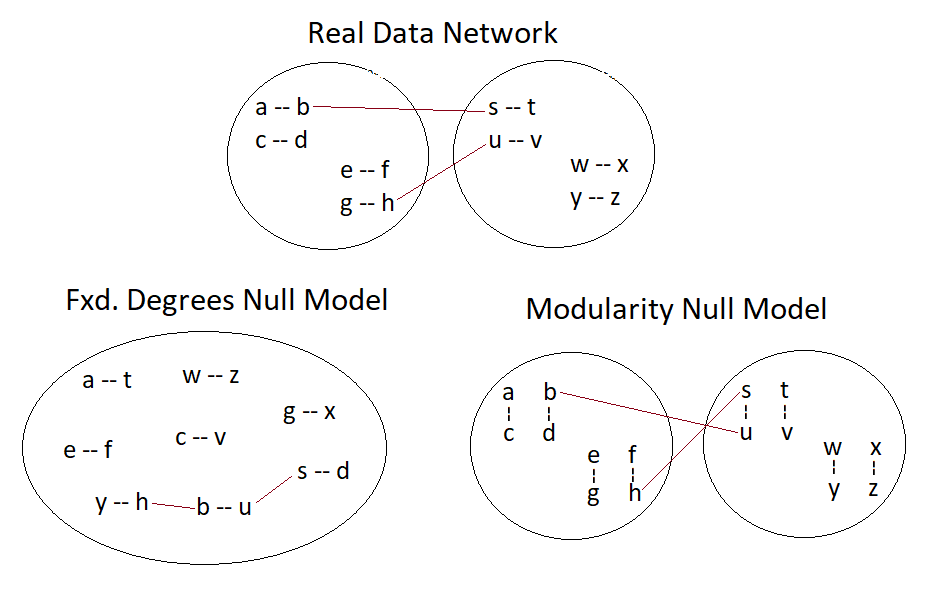
\includegraphics[width=0.6\linewidth]{../images/cartoon-null-model-definitions.png}}
		\caption{Formation of Different Null Models.}
		\label{figure-null_models}
	\end{center}
\end{figure}

Our analysis pipeline considers two types of randomised graphs for our association networks: \ac{nmd} and \ac{nmm}, as shown in Fig.~\ref{figure-null_models}. In \acs{nmd}, all edges that belong to the real network are shuffled in a pairwise fashion by keeping the original degrees sequence which allows conserving any possible skewed degree distribution in the real network~\cite{Maslov910, Fretter2012, FORTUNATO201075}. In \acs{nmm}, intra-edges and inter-edges among modules are shuffled separately by preserving the original degrees sequence~\cite{Fretter2012}. We should emphasise an essential detail in our design decision that might affect the results; \acs{nmm} keeps inter-edges from different module pairs together while the shuffling process, even if there are more than two modules in the real network. However, some module pairs might be strongly interconnected in most realistic situations, while the others are almost not linked to each other.
 \begin{figure}[!ht]
	\begin{center}
		\makebox[\textwidth]{
			\centering
			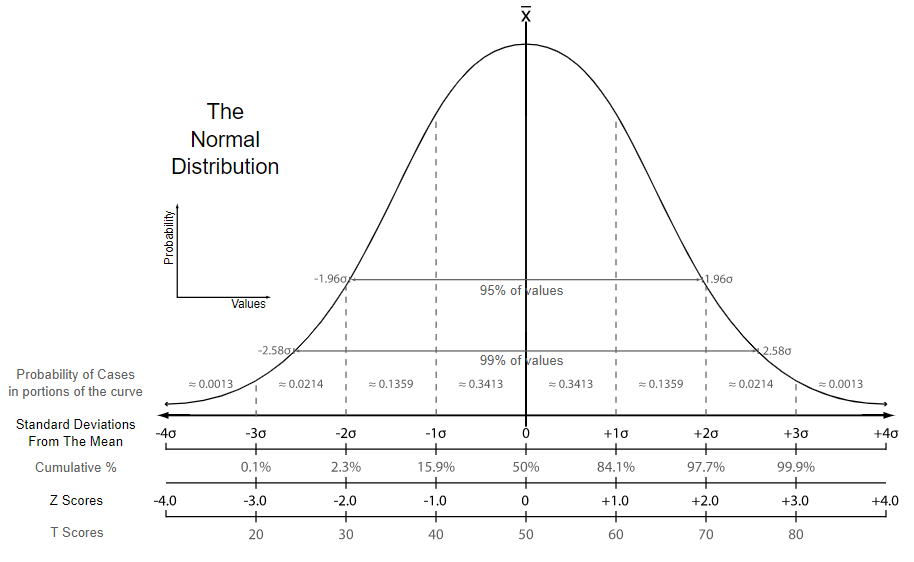
\includegraphics[width=0.85\linewidth]{../images/methodology-network-metrics-analysis-normal_distribution.png}}
		\caption{Chart Comparing the Various Grading Methods in A Normal Distribution.}
		\label{figure-normal_distribution}
	\end{center}
\end{figure}


One thousand random graphs concerning the respective null model constraints are created, and their modularity values are computed to compare with the real network. The histogram of resulted modularity values converges to a normal distribution like the one shown in Fig.~\ref{figure-normal_distribution}~\cite{normaldistribution}. One can quantify the real network randomness in the context of the respective null model by computing the \acl{zscore} (the so-called \acs{zscore}), $z$, as
\begin{equation} %\tag{2}
	z = \frac{Q-\mu}{\sigma}.
	\label{zscore}
\end{equation} 
\myequations{Standard Score Formula} 

$Q$ is the modularity value for the real network; $\mu$ is the expectation value (mean) of $Q$ in the set of $1000$ randomised graphs. $\sigma$ is the standard deviation of $Q$ in the randomised graphs.

$z$ is the number of standard deviations by which the real network modularity value is below or above the expected value, $\mu$. The \acs{zscore} lower than $1$ or higher than $-1$ indicate that the real network is incidental; the \acs{zscore} between $1$ and $2$ or between $-2$ and $-1$ suggest that the real network is close to random characteristics. In contrast, the \acs{zscore} greater than $2$ or less than $-2$ indicate a significant deviation from randomness.

\acs{nmd} is the null model that gives information about the modularity since it destroys the modules in the real network while randomising it. \acs{nmm} is essentially the control null model to detect strange effects and whether it is meaningful to discuss modularity. Comparing a real modular network with \acs{nmm} random graphs will lead the \acs{zscore} to zero, no matter the actual modularity value. If the \acs{zscore} using \acs{nmm} is drastically away from zero, then the type of modularity in the real network graphs are somewhat different and very complicated.

In some networks, small groups of nodes organised by following a hierarchical rule~\cite{BARABASI2001559} form large groups displaying a high degree of clustering while the degree distribution follows a power law~\cite{Barabasi2003}. That hierarchical organisation of nodes creates a nested modularity structure in the networks, having modules within modules. That type of organisation is observed in several real networks like the World wide web, the Internet at the domain level, actor-network~\cite{Barabasi2003}, macaque \& cat cortical systems~\cite{Young2000} and the Escherichia coli metabolic network~\cite{Ravasz1551}. We assume that the real network has a complicated structure or hierarchical organisation since the randomising scheme would destroy the internal modularity of graph modules if the \acs{zscore} concerning \acs{nmm} is lower than $-2$ or higher than $2$. 

Table~\ref{Tab: z-score_range_def} summarises possible network structures, including our assumptions for the respective \acs{zscore} intervals under the effect of null model choice.

\begin{table}[ht!]
	\centering
	\setlength{\arrayrulewidth}{0.78pt}%
	\caption{Expected Network Structures with Respect to Null Models.}
	\begin{tabular}{|
			>{\columncolor[HTML]{FFFFC7}}c |c|c|}
		\hline
		\begin{tabular}[c]{@{}c@{}}Real\\Network\\Z-score\end{tabular} & \cellcolor[HTML]{FFFFC7}\begin{tabular}[c]{@{}c@{}}Conserving \\ Degrees Sequence \\ (NM-d)\end{tabular} & \cellcolor[HTML]{FFFFC7}\begin{tabular}[c]{@{}c@{}}Conserving \\ Degrees Sequence \\ and Modules (NM-m)\end{tabular} \\ \hline
		$z\leq-2$ & \begin{tabular}[c]{@{}c@{}}nonrandom,\\ non-modular\end{tabular} & \begin{tabular}[c]{@{}c@{}}hierarchical\end{tabular} \\ \hline
		$-2<z<2$ & \begin{tabular}[c]{@{}c@{}}random,\\ non-modular\end{tabular} & \begin{tabular}[c]{@{}c@{}}simple\end{tabular} \\ \hline
		$z\geq2$ & \begin{tabular}[c]{@{}c@{}}nonrandom,\\ modular\end{tabular} & \begin{tabular}[c]{@{}c@{}}hierarchical\end{tabular} \\ \hline
	\end{tabular}
	\label{Tab: z-score_range_def}
\end{table}
